\documentclass[11pt]{article}            % Report class in 11 points
\parindent0pt  \parskip10pt             % make block paragraphs
\usepackage{graphicx}
\usepackage{listings}
\graphicspath{ {images/} }
\usepackage{graphicx} %  graphics header file
\begin{document}
\begin{titlepage}
    \centering
  \vfill
    
\includegraphics[width=8cm]{uni_logo.png} \\ 
	\vskip2cm
    {\bfseries\Large
	Artificial Intelligence \\ (CS13217)\\
	
	\vskip2cm
	Lab Report 
	 
	\vskip2cm
	}    

\begin{center}
\begin{tabular}{ l l  } 

Name: & Anam bibi \\ 
Registration \#: & CSU-S15-118\\ 
Lab Report \#: & 04 \\ 
 Dated:& 6-04-2018\\ 
Submitted To:& Mr. Usman Ahmed\\ 

 %\hline
\end{tabular}
\end{center}
    \vfill
    The University of Lahore, Islamabad Campus\\
Department of Computer Science \& Information Technology
\end{titlepage}


    
    {\bfseries\Large
\centering
	Experiment \# 4 \\

Implementing Breath First Search\\
	
	}    
 \vskip1cm
 \textbf {Objective}\\  To understand and implement the breath first search.
 
 \textbf {Software Tool} \\
1. operating system window 10 \\
2. sublime version 3.0\\
3. Python\\

\section{Theory }              
Breadth-first search (BFS) is an algorithm for traversing or searching tree or graph data structures. It starts at the tree root  and explores the neighbor nodes first, before moving to the next level neighbours.BFS is similar to level order traversal in a tree, where we visit vertices in a level by level order. We specify a starting vertex S and start visiting vertices of the graph G from the vertex S. As a general graph can have cycles, we may visit the same vertex more than once. To solve this, we also maintain the state of each vertex. A vertex can be in one of three states, VISITED. The basic idea of breadth first search is to find the least number of edges between S and any other vertex in G. Starting from S, we visit vertices of distance k before visiting any vertex of distance k+1. For that purpose, define ds(v) to be the least number of edges between S and v in G. So, for vertices v that are not reachable from S we can have ds(v) = ∞. We can use a queue to store vertices in progress. \\
We solve these problems using a queue. Recall that a queue is a type of limited-access list. Data
is inserted to the back of the queue, but removed from the front. Refer to the end of the Data
Structures I lab for more details.
A queue is helpful in a BFS to keep track of the order in which we will visit the nodes. At
each level of the search, we add the neighbors of the current node to the queue. The collections
module in the Python standard library has a deque object that we will use as our queue.\\



\section{Task}  
\subsection{Procedure: Task 1 }
Steps of Breath First Search\\
1.	Push the root node in the Queue.\\
2.	Loop until the queue is empty.\\
3.	Remove the node from the Queue..\\
4.If the removed node has unvisited child nodes, mark them as visited and insert the unvisited children in the queue. \\     

\begin{figure*}
\centering
  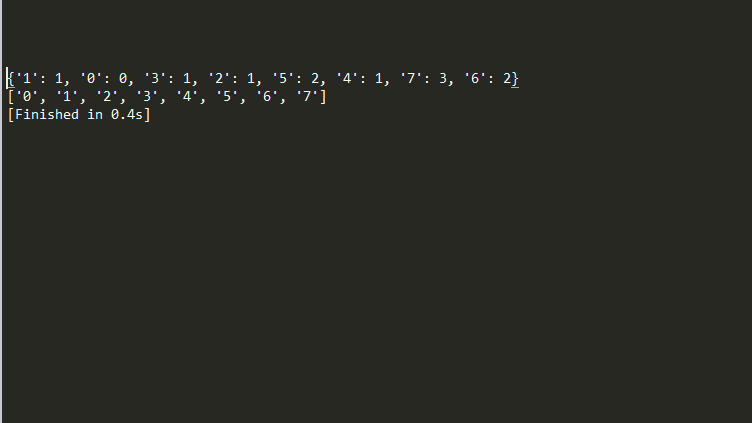
\includegraphics[width=12cm,height=6cm,keepaspectratio]{1.png}
\caption{Time Independent Feature Set}
\label{Figure:3}    
\end{figure*}
    

\begin{lstlisting}[language=Python]

 
graph = { 
    '0' : ['1','2','3','4'],
    '1' : ['0','5'],
    '2' : ['0','5'],
    '3' : ['0','6'],
    '4' : ['0','6'],
    '5' : ['1','2','7'],
    '6' : ['4','3','7'],
    '7' : ['6','5'],
    }

def bfs_connected_component(graph, start):
    explored = [] 
    queue = [start] 
    levels = {}        
    levels[start]= 0    
    visited= [start]    
    while queue:
        node = queue.pop(0) 
        explored.append(node)
        neighbours = graph[node]
        for neighbour in neighbours: 
            if neighbour not in visited:
                queue.append(neighbour)
                visited.append(neighbour)
                levels[neighbour]= levels[node]+1 
                
    print(levels)
    return explored
ans = bfs_connected_component(graph,'0') # returns ['0', '1', '2', '3', '4', '5', '6','7']
print(ans)
\end{lstlisting}

\section{Conclusion}  
Breadth First Search can be useful in graph traversal algorithms, one of its flaws is that it finds the shallowest goal node or station which doesn’t necessarily mean it’s the most optimal solution. Breadth First Search is only every optimal if for instance you happen to be in a scenario where all actions have the same cost.Breadth First graph traversal algorithms also happen to be very computationally demanding in the way that they calculate the shortest path.Breadth first search will never get trapped exploring the useless path forever.BFS-Graph is usually preferable, unless we know that there is a negligible number of duplicates in the given state space

 
\end{document}                          % The required last line
